%! Author = zhenxiang
%! Date = 23-3-23
\PassOptionsToPackage{quiet}{xeCJK}  % 抑制无意义的警告
% Preamble
\documentclass[11pt]{ctexart}

% Packages
\usepackage{amsmath}
% graphicx
\usepackage{graphicx}
% 页面设置
\usepackage{geometry}
\geometry{left=2.5cm, right=2.5cm, top=2.5cm, bottom=2.5cm}
% Document
\begin{document}

% CUDA PG Introduction
\section{Cuda-C-Programming-Guide Introduction Reading}
% 图片置于当前位置
\begin{figure}[h]
    \centering
    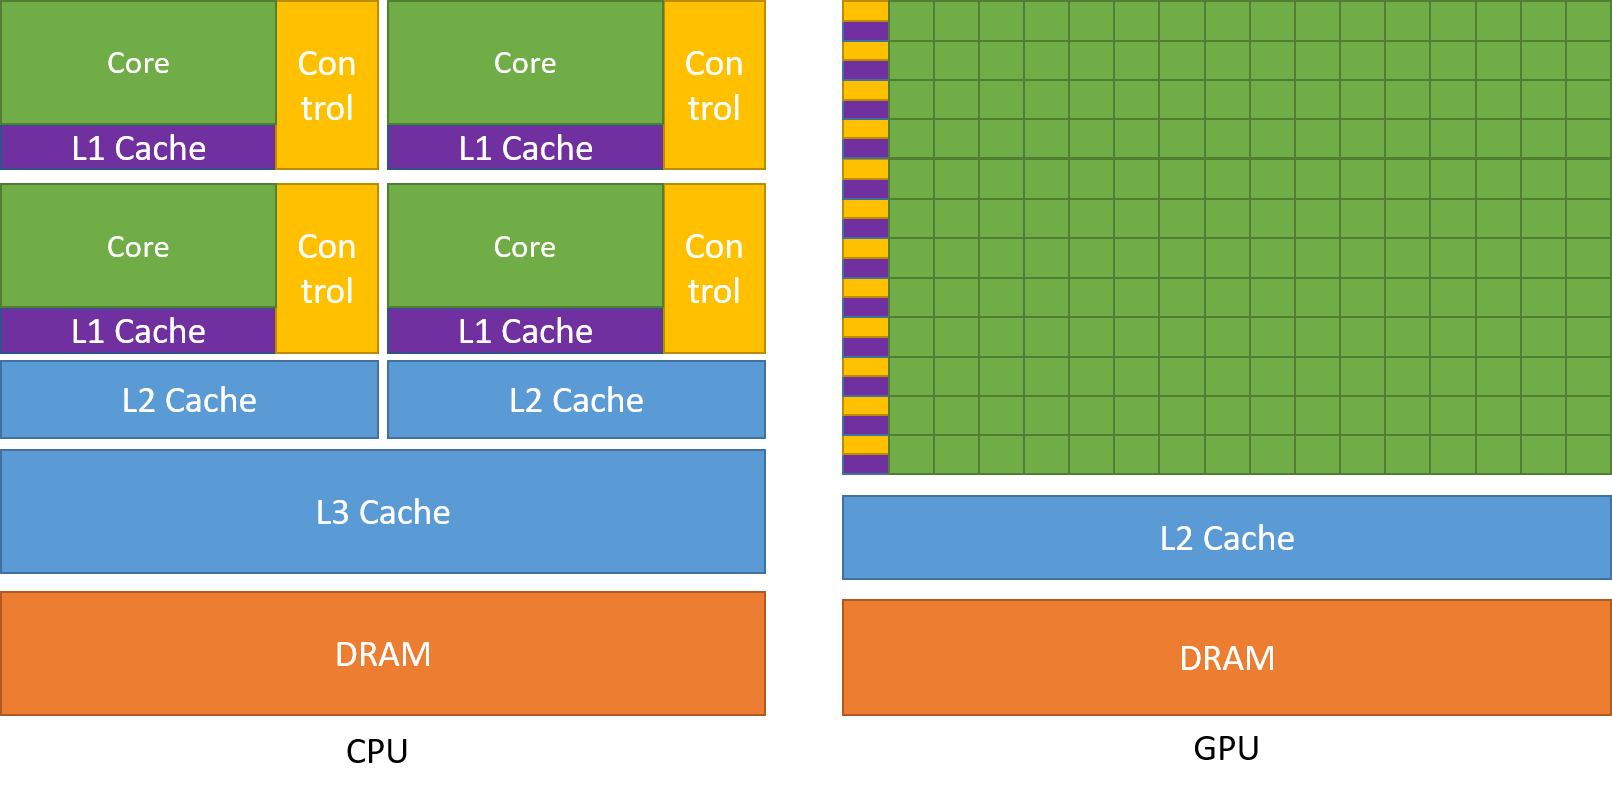
\includegraphics[width=0.8\textwidth]{photos/TheGPUDevotesMoreTransistorstoDataProcessing.png}
    \caption{The GPU Devotes More Transistors to Data Processing}
    \label{fig:1}
\end{figure}

The challenge is to develop application software that transparently scales its parallelism to leverage the increasing number of processor cores, much as 3D graphics applications transparently scale their parallelism to manycore GPUs with widely varying numbers of cores.\\

The CUDA parallel programming model is designed to overcome this challenge while maintaining a low learning curve for programmers familiar with standard programming languages such as C.\\

At its core are three key abstractions — \textbf{a hierarchy of thread groups}, \textbf{shared memories}, and \textbf{barrier synchronization} — that are simply exposed to the programmer as a minimal set of language extensions.
% 提供了细粒度的数据和线程并行性
These abstractions provide fine-grained data parallelism and thread parallelism, nested within coarse-grained data parallelism and task parallelism. \\

% 每个线程快可以以任何顺序、并发或串行地安排在GPU内的任何可用多处理器上,因此编译后的CUDA程序可以在任意数量的多处理器上执行,仅仅运行时系统需要直到物理多处理器计数。
This decomposition preserves language expressivity by allowing threads to cooperate when solving each sub-problem, and at the same time enables automatic scalability. Indeed, each block of threads can be scheduled on any of the available multiprocessors within a GPU, in any order, concurrently or sequentially, so that a compiled CUDA program can execute on any number of multiprocessors as illustrated by Figure 2, and only the runtime system needs to know the physical multiprocessor count.

% 图片置于当前位置
\begin{figure}[ht]
    \centering
    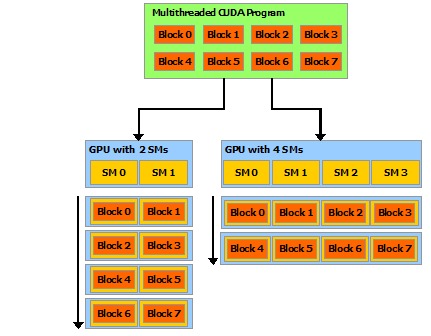
\includegraphics[width=0.8\textwidth]{photos/AutomaticScalability.png}
    \caption{Automatic Scalability}
    \label{fig:2}
\end{figure}

\newpage
\section{Programming Massively Parallel Processors}

Historically, most software developers have relied on the advances in hardware to
increase the speed of their sequential applications under the hood; the same software
simply runs faster as each new processor generation is introduced.\\

Now that all new microproces-
sors are parallel computers, the number of applications that need to be developed as
parallel programs has increased dramatically. There is now a great need for software
developers to learn about parallel programming, which is the focus of this book.\\
% 控制逻辑和高速缓存不对峰值计算吞吐量做出贡献是因为它们主要是针对提高顺序代码性能而设计的,而峰值计算吞吐量通常是通过并行执行多个指令或线程来实现的。控制逻辑和高速缓存可以提高单个线程的性能,但无法增加同时执行的指令数量或线程数量,因此不会对峰值计算吞吐量产生直接影响。

The design of a CPU is optimized for sequential code perfor-mance. It makes use of sophisticated control logic to allow instructions from a single
thread to execute in parallel or even out of their sequential order while maintaining
the appearance of sequential execution. More importantly, large cache memories are
provided to reduce the instruction and data access latencies of large complex appli-
cations. Neither control logic nor cache memories contribute to the peak calculation
throughput.\\

%降低延迟比增加吞吐量更昂贵,是因为降低延迟需要更多的硬件资源和更复杂的电路设计,这些都会增加芯片面积和功耗。例如,在处理器中引入更多的流水线级别可以降低指令执行的延迟,但是这样会增加流水线级别的数量和相关的控制逻辑,从而增加芯片面积和功耗。相反,增加吞吐量可以通过并行处理更多的任务来实现,而不需要增加每个任务的执行速度。因此,在GPU设计中,通常更注重增加吞吐量而不是降低延迟,以实现更高效的浮点运算。
%GPU设计中注重增加吞吐量而不是降低延迟的代价是可能会导致一些任务的响应时间变长。因为在处理大量线程时,单个线程的执行时间可能会变长,从而导致整个系统的响应时间变长。此外,由于GPU设计中的内存和算术单元通常具有长延迟,因此在某些应用场景中可能会出现性能瓶颈。因此,在实际应用中,需要根据具体的应用场景和需求,权衡吞吐量和延迟的优先级,以达到最佳的性能和响应时间。
The design philosophy of the GPUs has been shaped by the fast growing video
game industry that exerts tremendous economic pressure for the ability to perform a
massive number of floating-point calculations per video frame in advanced games.
This demand motivates GPU vendors to look for ways to maximize the chip area
and power budget dedicated to floating-point calculations. An important observa-
tion is that reducing latency is much more expensive than increasing throughput
in terms of power and chip area. Therefore, the prevailing solution is to optimize
for the execution throughput of massive numbers of threads. The design saves chip
area and power by allowing pipelined memory channels and arithmetic operations
to have long-latency. The reduced area and power of the memory access hardware
and arithmetic units allows the designers to have more of them on a chip and thus
increase the total execution throughput.\\

%现在应该清楚,GPU被设计为并行的吞吐量计算引擎,它们在一些CPU表现良好的任务上表现不佳。对于只有一个或非常少量线程的程序,具有较低操作延迟的CPU可以实现比GPU更高的性能。当一个程序有大量线程时,具有更高执行吞吐量的GPU可以实现比CPU更高的性能。因此,人们应该期望许多应用程序同时使用CPU和GPU,在CPU上执行顺序部分,在GPU上执行数值密集部分。这就是NVIDIA于2007年推出的CUDA编程模型的设计目的,支持应用程序的联合CPU-GPU执行。对于支持联合CPU-GPU执行的需求在更近期的编程模型中也得到了体现,如OpenCL(附录A)、OpenACC(见章节:使用OpenACC进行并行编程)和C++AMP(附录D)。
It should be clear now that GPUs are designed as parallel, throughput-oriented
computing engines and they will not perform well on some tasks on which CPUs are
designed to perform well. For programs that have one or very few threads, CPUs with
lower operation latencies can achieve much higher performance than GPUs. When
a program has a large number of threads, GPUs with higher execution throughput
can achieve much higher performance than CPUs. Therefore, one should expect that
many applications use both CPUs and GPUs, executing the sequential parts on the CPU and numerically intensive parts on the GPUs. This is why the CUDA program-
ming model, introduced by NVIDIA in 2007, is designed to support joint CPU–GPU
execution of an application. 1 The demand for supporting joint CPU–GPU execution is
further reflected in more recent programming models such as OpenCL (Appendix A),
OpenACC (see chapter: Parallel programming with OpenACC), and C++AMP
(Appendix D).\\

It is also important to note that speed is not the only decision factor when application developers choose the processors for running their applications. Several other
factors can be even more important. First and foremost, the processors of choice must
have a very large presence in the market place, referred to as the installed base of
the processor.\\

Another important decision factor is practical form factors and easy accessibility.\\

Yet another important consideration in selecting a processor for executing numeric computing applications is the level of support for IEEE Floating-Point Standard. The standard enables predictable results across processors from different vendors. \\

Researchers have achieved speedups of more than 100X for some applications.However, this is typically achieved only after extensive optimization and tuning after the algorithms have been enhanced so that more than 99.9\% of the application execu-tion time is in parallel execution. In practice, straightforward parallelization of applications often saturates the memory (DRAM) bandwidth, resulting in only about a 10X speedup. The trick is to figure out how to get around memory bandwidth limitations, which involves doing one of many transformations to utilize specialized GPU
on-chip memories to drastically reduce the number of accesses to the DRAM. One
must, however, further optimize the code to get around limitations such as limited
on-chip memory capacity.\\

What makes parallel programming hard? First and foremost, it can be challenging to design parallel algorithms
with the same level of algorithmic (computational) complexity as sequential algorithms. 

Second, the execution speed of many applications is limited by memory access speed. We refer to these applications as memory-bound, as opposed to compute
bound, which are limited by the number of instructions performed per byte of data.
Achieving high-performance parallel execution in memory-bound applications often requires novel methods for improving memory access speed.

Third, the execution speed of parallel programs is often more sensitive to the input data characteristics than their sequential counter parts. Many real world applications need to deal with inputs with widely varying characteristics, such as erratic or unpredictable data rates, and very high data rates. The performance of parallel programs can sometimes vary dramatically with these characteristics.

Fourth, many real world problems are most naturally described with mathematical recurrences. Parallelizing these problems often requires nonintuitive ways of thinking about the problem and may require redundant work during execution.

Fortunately, most of these challenges have been addressed by researchers in the past. There are also common patterns across application domains that allow us to apply solutions derived from one domain to others. This is the primary reason why we will be presenting key techniques for addressing these challenges in the context of important parallel computation patterns.\\


Those who are familiar with both OpenCL and CUDA know that there is a remarkable similarity between the key concepts and features of OpenCL and those of CUDA. That is, a CUDA programmer can learn OpenCL programming with
minimal effort. More importantly, virtually all techniques learned using CUDA can be easily applied to OpenCL programming.\\

第2章介绍了数据并行计算和CUDA C编程,期望读者具有C编程的先前经验。它首先将CUDA C介绍为一个简单的、小型的C扩展,支持异构CPU/GPU联合计算和广泛使用的单程序多数据(SPMD)并行编程模型。然后涵盖了(1)识别应用程序中需要并行化的部分的思考过程,(2)隔离并行化代码使用的数据,使用API函数在并行计算设备上分配内存,(3)使用API函数将数据传输到并行计算设备,(4)开发将由并行线程执行的内核函数,(5)启动内核函数以供并行线程执行,以及(6)最终使用API函数调用将数据传输回主机处理器。

虽然第2章的目标是教授足够的CUDA C编程模型概念,以便学生能够编写简单的并行CUDA C程序,但它实际上涵盖了开发基于任何并行编程模型的并行应用所需的几个基本技能。我们使用向量加法的运行示例来说明这些概念。在本书的后部分,我们还将CUDA与其他并行编程模型,包括OpenMP、OpenACC和OpenCL进行比较。

第3章介绍了CUDA的并行执行模型的更多细节。它提供了足够的洞察力,以便读者能够使用CUDA C实现复杂的计算,并推断出其CUDA代码的性能行为。

第4章“内存和数据局部性”专门介绍了可用于容纳CUDA变量以管理数据传递和提高程序执行速度的特殊内存。我们介绍了分配和使用这些内存的CUDA语言特性。适当使用这些内存可以大大提高数据访问吞吐量,并有助于缓解内存系统中的流量拥堵。

第5章“性能考虑”介绍了当前CUDA硬件中几个重要的性能考虑因素。特别是,它在线程执行、内存数据访问和资源分配的理想模式方面提供了更多细节。这些细节构成了程序员推断其计算和数据组织决策对性能影响的概念基础。

第6章“数值考虑”介绍了IEEE-754浮点数格式、精度和准确性的概念。它展示了不同的并行执行安排可能导致不同的输出值。它还教授了数值稳定性的概念和在并行算法中维护数值稳定性的实用技术。

第7章到第12章介绍了六种重要的并行计算模式,让读者更深入地了解并行编程技术和并行执行机制。第7章介绍了卷积和模板,这是经常使用的并行计算模式,需要仔细管理数据访问局部性。我们还利用这种模式介绍了现代GPU中的常量内存和缓存。第8章介绍了归约树和前缀和,这是一种重要的并行计算模式,可以将顺序计算转换为并行计算。我们还利用这种模式介绍了并行算法中的工作效率概念。第9章介绍了直方图,这是在大型数据集中广泛用于模式识别的模式。我们还涵盖了合并操作,在分治工作分区策略中广泛使用的模式。第10章介绍了稀疏矩阵计算,这是用于处理非常大的数据集的模式。本章介绍了重新排列数据以实现更有效的并行访问的概念:数据压缩、填充、排序、转置和规范化。第11章介绍了归并排序和动态输入数据识别和组织。第12章介绍了图算法以及如何在GPU编程中有效实现图搜索。

虽然这些章节基于CUDA,但它们帮助读者建立并行编程的基础。我们相信,人们通过具体的例子学习最有效。也就是说,我们必须首先在特定的编程模型的上下文中学习概念,这为我们提供了坚实的基础,以便将我们的知识应用于其他编程模型。在这样做的过程中,我们可以借鉴我们在CUDA模型中的具体经验。对CUDA模型的深入了解还使我们能够获得成熟经验,这将有助于我们学习可能与CUDA模型无关的概念。

第13章,CUDA动态并行性,介绍了动态并行性。这是GPU根据数据或程序结构动态创建自身工作的能力,而不是等待CPU专门启动内核。

第14章,应用案例研究-非笛卡尔MRI,第15章,应用案例研究-分子可视化和分析,第16章,应用案例研究-机器学习,是三个实际应用的案例研究,带领读者通过并行化和优化应用程序以获得显著加速的思考过程。对于每个应用,我们首先确定并行执行基本结构的替代方式,然后推理每个替代方式的优缺点。然后我们通过代码转换的步骤来实现高性能。这三章帮助读者将之前章节中的所有材料结合起来,为他们自己的应用开发项目做好准备。第14章,应用案例研究-非笛卡尔MRI,涵盖了非笛卡尔MRI重建,以及不规则数据如何影响程序。第15章,应用案例研究-分子可视化和分析,涵盖了分子可视化和分析。第16章,应用案例研究-机器学习,涵盖了深度学习,这是GPU计算中变得非常重要的领域。我们介绍了简介,并将更深入的讨论留给其他来源。

第17章,并行编程和计算思维,介绍了计算思维。它通过讨论组织程序的计算任务的概念,使其可以并行处理来介绍计算思维。我们首先讨论将抽象科学概念转化为计算任务的翻译过程,这是生成质量应用程序软件的重要第一步,无论是串行还是并行。然后讨论并行算法结构及其对应用程序性能的影响,这是基于CUDA性能调优经验的基础。虽然我们不涉及这些替代并行编程风格,但我们期望读者能够通过本书获得的基础知识学习任何一种风格的编程。我们还提供了一个高级别的案例研究,以展示创造性计算思维的机会。

第18章,编程异构计算集群,涵盖了CUDA编程在异构集群上,其中每个计算节点包括CPU和GPU。我们讨论了在CUDA旁边使用MPI来集成节点间计算和节点内计算以及由此产生的通信问题和实践。

第19章,使用OpenACC进行并行编程,涵盖了使用OpenACC进行并行编程。OpenACC是一个基于指令的高级编程方法,允许程序员标识和指定可以由编译器和/或其他工具并行化的代码区域。OpenACC是并行程序员入门的简便方法。

第20章,CUDA和GPU计算的更多内容和第21章,结论和展望,提供了总结性的言论和对高度并行处理器体系结构主要趋势的简要调查,以及这些趋势如何可能影响未来的并行编程。我们总结了我们的目标,并总结了这些章节如何相互配合以帮助实现这些目标。我们预测这些快速发展的高度并行计算将使其成为未来十年最令人兴奋的领域之一。

\end{document}